\documentclass[border=4pt]{standalone}
\usepackage{tikz}
\usepackage{xcolor}
\usetikzlibrary{arrows.meta, positioning}
\newcommand{\pillar}[1]{\textcolor{blue!55!black}{\footnotesize\itshape #1}}
\begin{document}
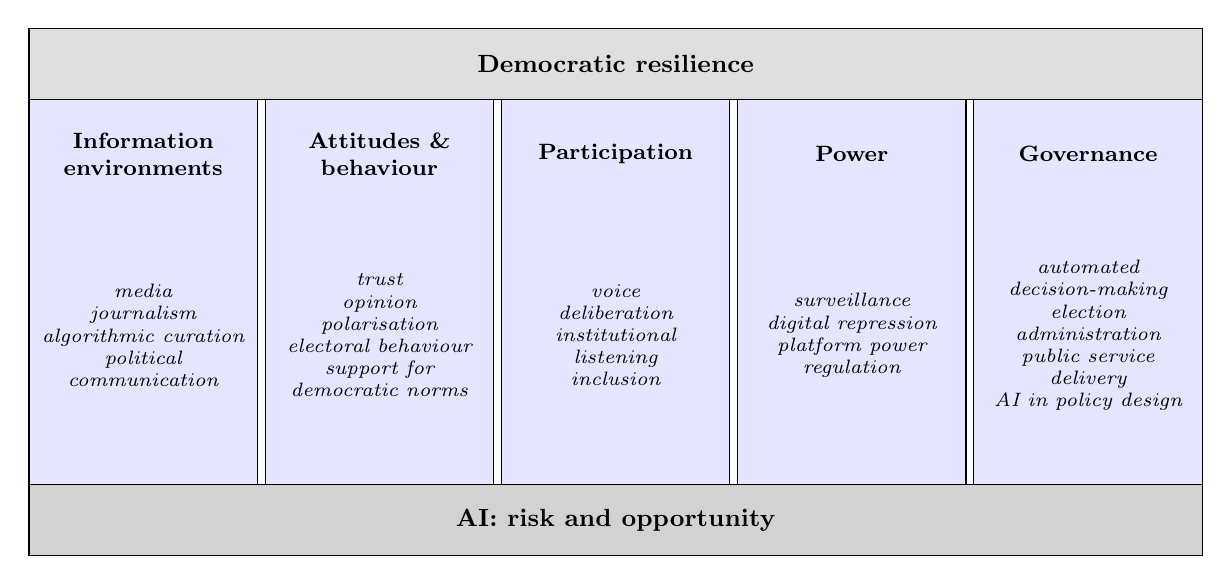
\begin{tikzpicture}[
  lbl/.style = {font=\bfseries\small, align=center},
  collbl/.style = {font=\bfseries\footnotesize, align=center, text width=2.7cm},
  sub/.style = {font=\scriptsize\itshape, align=center, text width=2.7cm, execute at begin node={\hyphenpenalty=10000\exhyphenpenalty=10000\relax}}
]
  % roof
  \draw[fill=gray!25] (-7.45,5.4) rectangle (7.45,6.3);
  \node[lbl] at (0,5.85) {Democratic resilience};

  % five columns, edges flush with the roof and base
  \foreach \x/\name/\items in {
    -6.0/{Information\\environments}/{media\\journalism\\algorithmic curation\\political communication},
    -3.0/{Attitudes \&\\behaviour}/{trust\\opinion\\polarisation\\electoral behaviour\\support for democratic norms},
    0/{Participation}/{voice\\deliberation\\institutional listening\\inclusion},
    3.0/{Power}/{surveillance\\digital repression\\platform power\\regulation},
    6.0/{Governance}/{automated decision-making\\election administration\\public service delivery\\AI in policy design}
  }{
    \draw[fill=blue!10] (\x-1.45,0.5) rectangle (\x+1.45,5.4);
    \node[collbl] at (\x,4.7) {\name};
    \node[sub] at (\x,2.4) {\items};
  }

  % base
  \draw[fill=gray!35] (-7.45,-0.4) rectangle (7.45,0.5);
  \node[lbl] at (0,0.05) {AI: risk and opportunity};
\end{tikzpicture}
\end{document}
